Sudoku is a popular logic puzzle invented by Howard Garns in the 70s but popularized and named in Japan in the following decade\cite{bib:sudoku}. To solve it, one usually applies a mixture of logic and trial and error. There are several variations but we will only concern ourselves with the classical Sudoku, played on a $9 \times 9$ grid where there exists a unique solution.

\subsection{Sudoku}
For convenience and as is often done in computing, we will draw our Cartesian coordinate system with the $y$-axis increasing downwards. We start with a few definitions in order to understand the game.

\begin{definition}
A \emph{cell} $(a,b)$ is the region $[a,a+1) \times [b,b+1) \subseteq \R^2$ where $a,b\in\N=\set{0,1,2,\ldots}$.
\end{definition}

\begin{definition}
A $n\times m$ \emph{grid} $\mathcal{G}$, where $(n,m) \in \Z^+\times\Z^+$, is the set of cells $\cset{(a,b)}{a < n \text{ and } b < m}$.
\end{definition}

\begin{definition}
A \emph{row} $r \in \{0,\ldots,m-1\}$ and \emph{column} $c\in\set{0,\ldots,n-1}$ in a $n\times m$ grid are the sets of cells $\cset{(i,r)}{0 \leq i < n}$ and $\cset{(c,j)}{0 \leq j < m}$ respectively. A \emph{block} in a $n^2 \times n^2$ grid is a set of cells $\cset{(x+i, y+j)}{i,j \in \set{0,1,\ldots,n-1}}$ where $x,y\in\set{0,n,\ldots,n^2-n}$ are fixed.
\end{definition}
In Figure \ref{fig:grid} we can see a $9\times9$ grid with examples of a cell, row, column and a block.

\begin{center}
  \begin{figure}[ht]
    \centering
    \def\scale{.65} % scale everything
    
    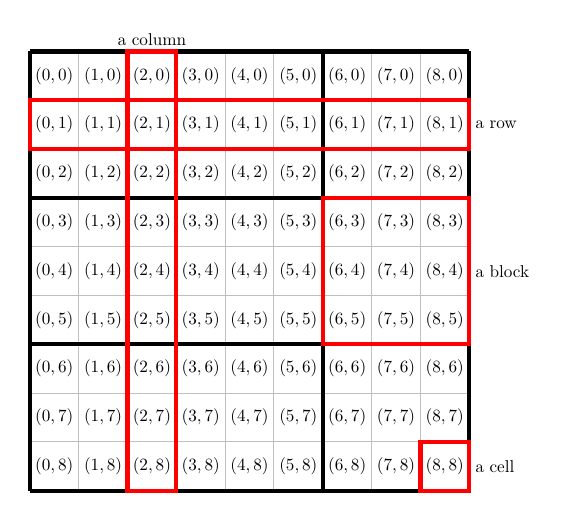
\begin{tikzpicture}[scale=\scale, every node/.style={scale=\scale}]
      \draw[gray!50] (0,0) grid (9,9);
      \draw[line width=0.55mm, scale=3] (0, 0) grid (3, 3);
      \foreach \x in {0,1,...,8} {
        \foreach \y in {0,1,...,8} {
            \draw (\x+.5,8.5-\y) node {$(\x,\y)$};
        }
      }
      \draw[line width=0.55mm, red] (8,0) rectangle (9,1);
      \draw[line width=0.55mm, red] (6,3) rectangle (9,6);
      \draw[line width=0.55mm, red] (0,7) rectangle (9,8);
      \draw[line width=0.55mm, red] (2,0) rectangle (3,9);
      \draw (9,.5) node[right] {a cell};
      \draw (9,4.5) node[right] {a block};
      \draw (9,7.5) node[right] {a row};
      \draw (2.5,9) node[above] {a column};
    \end{tikzpicture}
    \caption{A $9\times9$ grid and all of its subcomponents.}
    \label{fig:grid}
  \end{figure}
\end{center}

\begin{definition}
Given a $n^2 \times n^2$ grid $\mathcal{G}$ and two cells $c_1,c_2 \in \mathcal{G}$ where $c_1 \neq c_2$, then $c_1$ and $c_2$ are said to be \emph{peers} if there exists a row, column or block in $\mathcal{G}$ containing both.
\end{definition}

On a $9 \times 9$ grid, each cell will have exactly 20 peers, with 8 from a row, 8 from a column and 4 from a block when excluding the ones already counted by the row and column.

\begin{definition}
Let $\mathcal{G}$ be a $n^2\times n^2$ grid. A map $\phi: \mathcal{G} \mapsto \set{1,2,\ldots,n^2}$ is called a \emph{complete assignment} and a map $\varphi: \mathcal{C} \mapsto \set{1,2,\ldots,n^2}$ where $|\mathcal{C}| < |\mathcal{G}|$ and $\mathcal{C} \subseteq \mathcal{G}$ is called a partial assignment. In both cases, $\phi(c)$ and $\varphi(c)$ are called an \emph{assignment} of a cell $c\in\mathcal{G}$
\end{definition}

\begin{definition}
An assignment (either partial or complete) $\phi$ for a $n^2 \times n^2$ grid is said to be \emph{invalid} if there exists cells $c_1$ and $c_2$ in the domain of $\phi$ such that $c_1 \neq c_2$, $c_1$ and $c_2$ are peers and $\phi(c_1) = \phi(c_2)$. If an assignment is not invalid, it is \emph{valid}.
\end{definition}

As we only care about classical Sudoku we will shift focus from a general $n^2$ to the fixed number $9$ in terms of definitions.

\begin{definition}
A (classical) \emph{Sudoku puzzle} is a pair $(\mathcal{G}, \varphi)$ where $\mathcal{G}$ is a $9\times 9$ grid and $\varphi$ a valid partial assignment $\varphi: \mathcal{C} \to \set{1,2,\ldots,9}$ where $\mathcal{C}$ is a proper subset of $\mathcal{G}$ such that
\[
    |\cset{\phi}{\phi \text{ is a valid complete assignment and }\varphi(c) = \phi(c)\text{ for all }c\in\mathcal{C}}|=1.
\]
\end{definition}

We refer to this unique valid complete assignment as a \emph{solution} to a Sudoku puzzle. A Sudoku puzzle and its solution can be seen in Figure \ref{fig:sudpuzsol}.

\begin{center}
  \begin{figure}[ht]
    \centering
    \def\scale{.6} % scale everything
    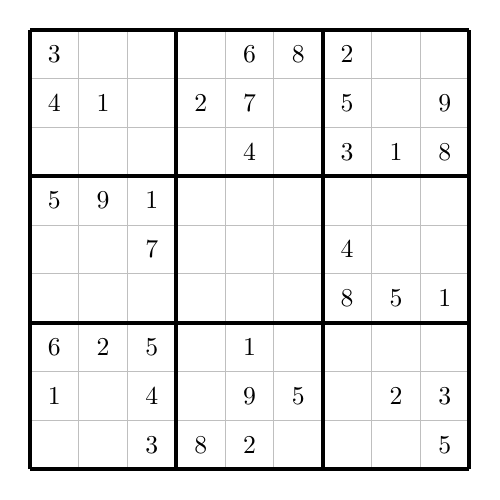
\begin{tikzpicture}[scale=\scale, every node/.style={scale=\scale}]
      \node[anchor=center,scale=1.5] at (0.5, 8.5) {$3$};
      \node[anchor=center,scale=1.5] at (4.5, 8.5) {$6$};
      \node[anchor=center,scale=1.5] at (5.5, 8.5) {$8$};
      \node[anchor=center,scale=1.5] at (6.5, 8.5) {$2$};
      \node[anchor=center,scale=1.5] at (0.5, 7.5) {$4$};
      \node[anchor=center,scale=1.5] at (1.5, 7.5) {$1$};
      \node[anchor=center,scale=1.5] at (3.5, 7.5) {$2$};
      \node[anchor=center,scale=1.5] at (4.5, 7.5) {$7$};
      \node[anchor=center,scale=1.5] at (6.5, 7.5) {$5$};
      \node[anchor=center,scale=1.5] at (8.5, 7.5) {$9$};
      \node[anchor=center,scale=1.5] at (4.5, 6.5) {$4$};
      \node[anchor=center,scale=1.5] at (6.5, 6.5) {$3$};
      \node[anchor=center,scale=1.5] at (7.5, 6.5) {$1$};
      \node[anchor=center,scale=1.5] at (8.5, 6.5) {$8$};
      \node[anchor=center,scale=1.5] at (0.5, 5.5) {$5$};
      \node[anchor=center,scale=1.5] at (1.5, 5.5) {$9$};
      \node[anchor=center,scale=1.5] at (2.5, 5.5) {$1$};
      \node[anchor=center,scale=1.5] at (2.5, 4.5) {$7$};
      \node[anchor=center,scale=1.5] at (6.5, 4.5) {$4$};
      \node[anchor=center,scale=1.5] at (6.5, 3.5) {$8$};
      \node[anchor=center,scale=1.5] at (7.5, 3.5) {$5$};
      \node[anchor=center,scale=1.5] at (8.5, 3.5) {$1$};
      \node[anchor=center,scale=1.5] at (0.5, 2.5) {$6$};
      \node[anchor=center,scale=1.5] at (1.5, 2.5) {$2$};
      \node[anchor=center,scale=1.5] at (2.5, 2.5) {$5$};
      \node[anchor=center,scale=1.5] at (4.5, 2.5) {$1$};
      \node[anchor=center,scale=1.5] at (0.5, 1.5) {$1$};
      \node[anchor=center,scale=1.5] at (2.5, 1.5) {$4$};
      \node[anchor=center,scale=1.5] at (4.5, 1.5) {$9$};
      \node[anchor=center,scale=1.5] at (5.5, 1.5) {$5$};
      \node[anchor=center,scale=1.5] at (7.5, 1.5) {$2$};
      \node[anchor=center,scale=1.5] at (8.5, 1.5) {$3$};
      \node[anchor=center,scale=1.5] at (2.5, 0.5) {$3$};
      \node[anchor=center,scale=1.5] at (3.5, 0.5) {$8$};
      \node[anchor=center,scale=1.5] at (4.5, 0.5) {$2$};
      \node[anchor=center,scale=1.5] at (8.5, 0.5) {$5$};
      \draw[gray!50] (0,0) grid (9,9);
      \draw[line width=0.55mm, scale=3] (0, 0) grid (3, 3);
    \end{tikzpicture}
    \hspace{1cm}
    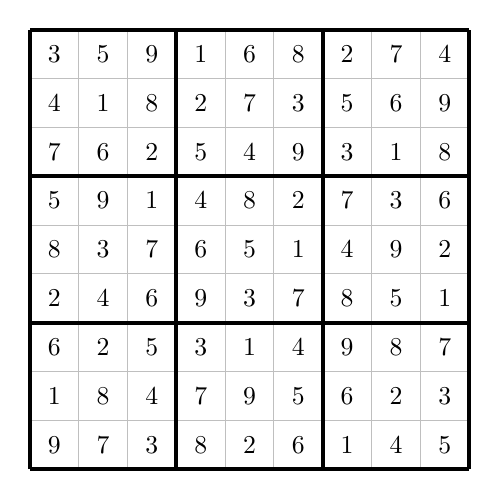
\begin{tikzpicture}[scale=\scale, every node/.style={scale=\scale}]
      \node[anchor=center,scale=1.5] at (0.5, 8.5) {$3$};
      \node[anchor=center,scale=1.5] at (1.5, 8.5) {$5$};
      \node[anchor=center,scale=1.5] at (2.5, 8.5) {$9$};
      \node[anchor=center,scale=1.5] at (3.5, 8.5) {$1$};
      \node[anchor=center,scale=1.5] at (4.5, 8.5) {$6$};
      \node[anchor=center,scale=1.5] at (5.5, 8.5) {$8$};
      \node[anchor=center,scale=1.5] at (6.5, 8.5) {$2$};
      \node[anchor=center,scale=1.5] at (7.5, 8.5) {$7$};
      \node[anchor=center,scale=1.5] at (8.5, 8.5) {$4$};
      \node[anchor=center,scale=1.5] at (0.5, 7.5) {$4$};
      \node[anchor=center,scale=1.5] at (1.5, 7.5) {$1$};
      \node[anchor=center,scale=1.5] at (2.5, 7.5) {$8$};
      \node[anchor=center,scale=1.5] at (3.5, 7.5) {$2$};
      \node[anchor=center,scale=1.5] at (4.5, 7.5) {$7$};
      \node[anchor=center,scale=1.5] at (5.5, 7.5) {$3$};
      \node[anchor=center,scale=1.5] at (6.5, 7.5) {$5$};
      \node[anchor=center,scale=1.5] at (7.5, 7.5) {$6$};
      \node[anchor=center,scale=1.5] at (8.5, 7.5) {$9$};
      \node[anchor=center,scale=1.5] at (0.5, 6.5) {$7$};
      \node[anchor=center,scale=1.5] at (1.5, 6.5) {$6$};
      \node[anchor=center,scale=1.5] at (2.5, 6.5) {$2$};
      \node[anchor=center,scale=1.5] at (3.5, 6.5) {$5$};
      \node[anchor=center,scale=1.5] at (4.5, 6.5) {$4$};
      \node[anchor=center,scale=1.5] at (5.5, 6.5) {$9$};
      \node[anchor=center,scale=1.5] at (6.5, 6.5) {$3$};
      \node[anchor=center,scale=1.5] at (7.5, 6.5) {$1$};
      \node[anchor=center,scale=1.5] at (8.5, 6.5) {$8$};
      \node[anchor=center,scale=1.5] at (0.5, 5.5) {$5$};
      \node[anchor=center,scale=1.5] at (1.5, 5.5) {$9$};
      \node[anchor=center,scale=1.5] at (2.5, 5.5) {$1$};
      \node[anchor=center,scale=1.5] at (3.5, 5.5) {$4$};
      \node[anchor=center,scale=1.5] at (4.5, 5.5) {$8$};
      \node[anchor=center,scale=1.5] at (5.5, 5.5) {$2$};
      \node[anchor=center,scale=1.5] at (6.5, 5.5) {$7$};
      \node[anchor=center,scale=1.5] at (7.5, 5.5) {$3$};
      \node[anchor=center,scale=1.5] at (8.5, 5.5) {$6$};
      \node[anchor=center,scale=1.5] at (0.5, 4.5) {$8$};
      \node[anchor=center,scale=1.5] at (1.5, 4.5) {$3$};
      \node[anchor=center,scale=1.5] at (2.5, 4.5) {$7$};
      \node[anchor=center,scale=1.5] at (3.5, 4.5) {$6$};
      \node[anchor=center,scale=1.5] at (4.5, 4.5) {$5$};
      \node[anchor=center,scale=1.5] at (5.5, 4.5) {$1$};
      \node[anchor=center,scale=1.5] at (6.5, 4.5) {$4$};
      \node[anchor=center,scale=1.5] at (7.5, 4.5) {$9$};
      \node[anchor=center,scale=1.5] at (8.5, 4.5) {$2$};
      \node[anchor=center,scale=1.5] at (0.5, 3.5) {$2$};
      \node[anchor=center,scale=1.5] at (1.5, 3.5) {$4$};
      \node[anchor=center,scale=1.5] at (2.5, 3.5) {$6$};
      \node[anchor=center,scale=1.5] at (3.5, 3.5) {$9$};
      \node[anchor=center,scale=1.5] at (4.5, 3.5) {$3$};
      \node[anchor=center,scale=1.5] at (5.5, 3.5) {$7$};
      \node[anchor=center,scale=1.5] at (6.5, 3.5) {$8$};
      \node[anchor=center,scale=1.5] at (7.5, 3.5) {$5$};
      \node[anchor=center,scale=1.5] at (8.5, 3.5) {$1$};
      \node[anchor=center,scale=1.5] at (0.5, 2.5) {$6$};
      \node[anchor=center,scale=1.5] at (1.5, 2.5) {$2$};
      \node[anchor=center,scale=1.5] at (2.5, 2.5) {$5$};
      \node[anchor=center,scale=1.5] at (3.5, 2.5) {$3$};
      \node[anchor=center,scale=1.5] at (4.5, 2.5) {$1$};
      \node[anchor=center,scale=1.5] at (5.5, 2.5) {$4$};
      \node[anchor=center,scale=1.5] at (6.5, 2.5) {$9$};
      \node[anchor=center,scale=1.5] at (7.5, 2.5) {$8$};
      \node[anchor=center,scale=1.5] at (8.5, 2.5) {$7$};
      \node[anchor=center,scale=1.5] at (0.5, 1.5) {$1$};
      \node[anchor=center,scale=1.5] at (1.5, 1.5) {$8$};
      \node[anchor=center,scale=1.5] at (2.5, 1.5) {$4$};
      \node[anchor=center,scale=1.5] at (3.5, 1.5) {$7$};
      \node[anchor=center,scale=1.5] at (4.5, 1.5) {$9$};
      \node[anchor=center,scale=1.5] at (5.5, 1.5) {$5$};
      \node[anchor=center,scale=1.5] at (6.5, 1.5) {$6$};
      \node[anchor=center,scale=1.5] at (7.5, 1.5) {$2$};
      \node[anchor=center,scale=1.5] at (8.5, 1.5) {$3$};
      \node[anchor=center,scale=1.5] at (0.5, 0.5) {$9$};
      \node[anchor=center,scale=1.5] at (1.5, 0.5) {$7$};
      \node[anchor=center,scale=1.5] at (2.5, 0.5) {$3$};
      \node[anchor=center,scale=1.5] at (3.5, 0.5) {$8$};
      \node[anchor=center,scale=1.5] at (4.5, 0.5) {$2$};
      \node[anchor=center,scale=1.5] at (5.5, 0.5) {$6$};
      \node[anchor=center,scale=1.5] at (6.5, 0.5) {$1$};
      \node[anchor=center,scale=1.5] at (7.5, 0.5) {$4$};
      \node[anchor=center,scale=1.5] at (8.5, 0.5) {$5$};
      \draw[gray!50] (0,0) grid (9,9);
      \draw[line width=0.55mm, scale=3] (0, 0) grid (3, 3);
    \end{tikzpicture}
    \caption{A Sudoku puzzle and its solution.}
    \label{fig:sudpuzsol}
  \end{figure}
\end{center}

In essence, a Sudoku puzzle is a $9$-coloring problem where each color represents a number from $\set{1,2,\ldots,9}$, the cells are vertices and two vertices have an edge between them if they are peers and we are provided with a few colorings such that the remaining ones can only be colored in a single way.


\subsection{Sudoku as a CSP}
There are different ways to model Sudoku as a CSP. We will let all cells be variables, regardless of them being assigned or not, and instead reduce the domains to singleton sets for assigned cells. The constraints are all non-equal binary constraints between peers. Alternatively, we could have omitted the assigned cells from the variables and introduced some unary constraints on their peers.
\begin{definition}
A \emph{Sudoku CSP} for a Sudoku puzzle with partial assignment $\varphi: \mathcal{C} \to \set{1,2,\ldots,9}$ is a triple $(X,D,C)$ with \emph{variables} $X=\set{x_0,x_1,\ldots,x_{80}}$ where $x_i$ represents the cell $c_i = \left(i \pmod 9, \lfloor i/9  \rfloor\right)$, \emph{domains}
\[
    D_i = \begin{cases}\set{\varphi(c_i)} & \mbox{ if $c_i \in \mathcal{C}$}\\\set{1,2,\ldots,9} & \mbox{ otherwise }\end{cases}
\]
and \emph{constraints} $C = \cset{(i,j)}{i < j \text{ and } c_i \text{ and } c_j \text{ are peers}}$  for $i,j\in\set{0,1,\ldots,80}$.
\end{definition}

Our goal is to find the assignment of the variables, $(v_0,v_2,\ldots,v_{80}) \in D_0 \times D_1 \times \cdots \times D_{80}$, such that all constraints are satisfied. An element $(i,j)\in C$ represents the constraint that $x_i$ and $x_j$ must not be equal. Note that we restrict our constraints to include only ordered pairs as non-equality is a reflexive relation over $\set{1,2,\ldots,9}$. For example $C$ would contain $(x_2,x_{38})$ but not $(x_{38},x_2)$. Figure \ref{fig:variables} shows all variables of a Sudoku CSP on a grid as well as all constraints involving the variable $x_{38}$. The green cells represent the peers of $x_{38}$ where $x_{38}$ would be the second element of the pair in $C$, the blue cells represent the peers where $x_{38}$ would be the first one and finally, $x_{38}$ itself is highlighted with red. Since each variable has 20 peers and the order does not matter (with regards to counting), there are $\frac{9\cdot9\cdot20}{2} = \frac{1620}{2} = 810$ unique constraints in the entire CSP. We divide by 2 to avoid counting each pair twice.

\begin{center}
  \begin{figure}[ht]
    \centering
    \def\scale{.62} % scale everything
    
    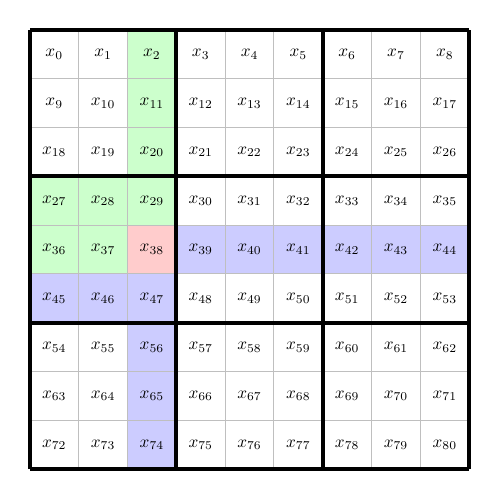
\begin{tikzpicture}[scale=\scale, every node/.style={scale=\scale}]
        \fill[green!20] (2,5) rectangle (3,9);
        \fill[green!20] (0,4) rectangle (2,6);
        \fill[blue!20] (0,3) rectangle (3,4);
        \fill[blue!20] (3,4) rectangle (9,5);
        \fill[blue!20] (2,0) rectangle (3,3);
        \fill[red!20] (2,4) rectangle (3,5);
      \draw[gray!50] (0,0) grid (9,9);
      \draw[line width=0.55mm, scale=3] (0, 0) grid (3, 3);
      \foreach \x in {0,1,...,80} {
            \draw ({0.5+Mod(\x,9)}, {8.5-int(\x/9)}) node {$x_{\x}$};
      }
    \end{tikzpicture}
    \caption{The variables of Sudoku and the constraints involving the variable $x_{38}$.}
    \label{fig:variables}
  \end{figure}
\end{center}

\begin{definition}
A Sudoku CSP $(X,D,C)$ is \emph{arc-consistent} if for all variables $x_i,x_j \in X$ where $x_i$ and $x_j$ represent non-equal cells that are peers and for all values $v\in D_i$ the set $D_j \setminus \set{v}$ is not empty.
\end{definition}
